\documentclass[a4paper,oneside,12pt]{extreport}

\usepackage{mmap}
\usepackage[T2A]{fontenc}
\usepackage[utf8]{inputenc}
\usepackage[english,russian]{babel}

\renewcommand{\ttdefault}{PTMono-TLF}

% Текст отчёта следует печатать, соблюдая следующие размеры полей:
% левое — 30 мм, правое — 15 мм, верхнее и нижнее — 20 мм.
\usepackage[left=20mm, right=15mm, top=15mm, bottom=15mm]{geometry}

% \setlength{\parindent}{1.25cm} % Абзацный отступ

\usepackage{setspace}
% \onehalfspacing % Полуторный интервал

\frenchspacing % Равномерные пробелы
\usepackage{indentfirst} % Красная строка

\usepackage{microtype}
\sloppy

\usepackage{titlesec}
\titlespacing*{\chapter}{0pt}{-30pt}{8pt}
\titlespacing*{\section}{\parindent}{*4}{*4}
\titlespacing*{\subsection}{\parindent}{*4}{*4}
\titleformat{\chapter}{\LARGE\bfseries}{\thechapter}{20pt}{\LARGE\bfseries}
\titleformat{\section}{\Large\bfseries}{\thesection}{40pt}{\Large\bfseries}

\usepackage{graphicx}
\usepackage{caption}
\usepackage{float}

\usepackage[unicode,pdftex]{hyperref}
\hypersetup{hidelinks}

%% begin title
\usepackage{wrapfig}

\makeatletter
	\def\vhrulefill#1{\leavevmode\leaders\hrule\@height#1\hfill \kern\z@}
\makeatother
%% end title

%% begin code
\usepackage{listings}
\usepackage{listingsutf8}
\usepackage{xcolor}

\lstset{language=Matlab,%
    %basicstyle=\color{red},
    breaklines=true,%
    morekeywords={matlab2tikz},
    keywordstyle=\color{blue},%
    morekeywords=[2]{1}, keywordstyle=[2]{\color{black}},
    identifierstyle=\color{black},%
    stringstyle=\color{mylilas},
    commentstyle=\color{mygreen},%
    showstringspaces=false,%without this there will be a symbol in the places where there is a space
    numbers=left,%
    numberstyle={\tiny \color{black}},% size of the numbers
    numbersep=9pt, % this defines how far the numbers are from the text
    emph=[1]{for,end,break},emphstyle=[1]\color{red}, %some words to emphasise
    %emph=[2]{word1,word2}, emphstyle=[2]{style},    
    literate={Ö}{{\"O}}1
    {Ä}{{\"A}}1
    {Ü}{{\"U}}1
    {ß}{{\ss}}1
    {ü}{{\"u}}1
    {ä}{{\"a}}1
    {ö}{{\"o}}1
    {~}{{\textasciitilde}}1
    {а}{{\selectfont\char224}}1
    {б}{{\selectfont\char225}}1
    {в}{{\selectfont\char226}}1
    {г}{{\selectfont\char227}}1
    {д}{{\selectfont\char228}}1
    {е}{{\selectfont\char229}}1
    {ё}{{\"e}}1
    {ж}{{\selectfont\char230}}1
    {з}{{\selectfont\char231}}1
    {и}{{\selectfont\char232}}1
    {й}{{\selectfont\char233}}1
    {к}{{\selectfont\char234}}1
    {л}{{\selectfont\char235}}1
    {м}{{\selectfont\char236}}1
    {н}{{\selectfont\char237}}1
    {о}{{\selectfont\char238}}1
    {п}{{\selectfont\char239}}1
    {р}{{\selectfont\char240}}1
    {с}{{\selectfont\char241}}1
    {т}{{\selectfont\char242}}1
    {у}{{\selectfont\char243}}1
    {ф}{{\selectfont\char244}}1
    {х}{{\selectfont\char245}}1
    {ц}{{\selectfont\char246}}1
    {ч}{{\selectfont\char247}}1
    {ш}{{\selectfont\char248}}1
    {щ}{{\selectfont\char249}}1
    {ъ}{{\selectfont\char250}}1
    {ы}{{\selectfont\char251}}1
    {ь}{{\selectfont\char252}}1
    {э}{{\selectfont\char253}}1
    {ю}{{\selectfont\char254}}1
    {я}{{\selectfont\char255}}1
    {А}{{\selectfont\char192}}1
    {Б}{{\selectfont\char193}}1
    {В}{{\selectfont\char194}}1
    {Г}{{\selectfont\char195}}1
    {Д}{{\selectfont\char196}}1
    {Е}{{\selectfont\char197}}1
    {Ё}{{\"E}}1
    {Ж}{{\selectfont\char198}}1
    {З}{{\selectfont\char199}}1
    {И}{{\selectfont\char200}}1
    {Й}{{\selectfont\char201}}1
    {К}{{\selectfont\char202}}1
    {Л}{{\selectfont\char203}}1
    {М}{{\selectfont\char204}}1
    {Н}{{\selectfont\char205}}1
    {О}{{\selectfont\char206}}1
    {П}{{\selectfont\char207}}1
    {Р}{{\selectfont\char208}}1
    {С}{{\selectfont\char209}}1
    {Т}{{\selectfont\char210}}1
    {У}{{\selectfont\char211}}1
    {Ф}{{\selectfont\char212}}1
    {Х}{{\selectfont\char213}}1
    {Ц}{{\selectfont\char214}}1
    {Ч}{{\selectfont\char215}}1
    {Ш}{{\selectfont\char216}}1
    {Щ}{{\selectfont\char217}}1
    {Ъ}{{\selectfont\char218}}1
    {Ы}{{\selectfont\char219}}1
    {Ь}{{\selectfont\char220}}1
    {Э}{{\selectfont\char221}}1
    {Ю}{{\selectfont\char222}}1
    {Я}{{\selectfont\char223}}1
    {і}{{\selectfont\char105}}1
    {ї}{{\selectfont\char168}}1
    {є}{{\selectfont\char185}}1
    {ґ}{{\selectfont\char160}}1
    {І}{{\selectfont\char73}}1
    {Ї}{{\selectfont\char136}}1
    {Є}{{\selectfont\char153}}1
    {Ґ}{{\selectfont\char128}}1
}

%% end code

%% begin theorem
\usepackage{amsthm}

\makeatletter
\newtheoremstyle{indented}
	{}% measure of space to leave above the theorem
	{}% measure of space to leave below the theorem
	{}% name of font to use in the body of the theorem
	{\parindent}% measure of space to indent
	{\bfseries}% name of head font
	{.}% punctuation between head and body
	{ }% space after theorem head; " " = normal interword space
	{}% header specification (empty for default)
\makeatother

\theoremstyle{indented}

\newtheorem{definition}{Определение}[section]
\newtheorem{remark}{Замечание}[section]
%% end theorem


\usepackage{amsmath, amsfonts, amssymb}

\renewcommand\thesection{\arabic{section}}
\renewcommand\thesubsection{\thesection.\arabic{subsection}}

\begin{document}
\paragraph{Цель работы:} построение доверительных интервалов для математического ожидания и дисперсии нормальной случайной величины.

\paragraph{Содержание работы}

\begin{enumerate}
	\item Для выборки объема $n$ из нормальной генеральной совокупности $X$ реализовать в виде программы на ЭВМ
	\begin{itemize}
		\item вычисление точечных оценок $\hat\mu(\vec X_n)$ и $S^2(\vec X_n)$ математического ожидания $MX$ и дисперсии $DX$ соответственно;
		\item вычисление нижней и верхней границ $\underline\mu(\vec X_n)$, $\overline\mu(\vec X_n)$ для $\gamma$-доверительного интервала для математического ожидания $MX$;
		\item вычисление нижней и верхней границ $\underline\sigma^2(\vec X_n)$, $\overline\sigma^2(\vec X_n)$ для $\gamma$-доверительного интервала для дисперсии $DX$;
	\end{itemize}
	\item вычислить $\hat\mu$ и $S^2$ для выборки из индивидуального варианта;
	\item для заданного пользователем уровня доверия $\gamma$ и $N$ – объёма выборки из индивидуального варианта:
	\begin{itemize}
		\item на координатной плоскости $Oyn$ построить прямую $y = \hat\mu(\vec{x_N})$, также графики функций $y = \hat\mu(\vec x_n)$, $y = \underline\mu(\vec x_n)$ и $y = \overline\mu(\vec x_n)$ как функций объема $n$ выборки, где $n$ изменяется от 1 до $N$;
		\item на другой координатной плоскости $Ozn$ построить прямую $z = S^2(\vec{x_N})$, также графики функций $z = S^2(\vec x_n)$, $z = \underline\sigma^2(\vec x_n)$ и $z = \overline\sigma^2(\vec x_n)$ как функций объема $n$ выборки, где $n$ изменяется от 1 до $N$.
	\end{itemize}
\end{enumerate}

\pagebreak
\section{Вариант 21, выборка}
$\vec{x} = ( 

~~~~~~~-14.34, -16.97, -14.09, -14.74, -16.69, -13.85, -15.55, -14.62, -13.30, -15.52,

~~~~~~~-14.75, -16.51, -17.15, -16.87, -15.06, -13.60, -14.48, -14.71, -14.17, -13.88,

~~~~~~~-14.55, -15.37, -14.81, -16.05, -17.06, -15.86, -15.12, -15.98, -14.16, -15.81,

~~~~~~~-15.06, -16.19, -16.22, -16.19, -14.87, -15.62, -15.86, -15.25, -16.34, -14.44,

~~~~~~~-14.72, -15.17, -15.24, -14.44, -15.93, -14.87, -16.53, -15.76, -15.12, -12.91,

~~~~~~~-16.06, -16.06, -14.89, -15.57, -13.59, -16.84, -13.88, -14.33, -15.45, -16.58,

~~~~~~~-16.05, -14.34, -13.55, -16.78, -14.15, -14.28, -14.40, -13.98, -16.23, -15.35,

~~~~~~~-14.77, -15.61, -15.59, -15.64, -14.76, -17.18, -15.13, -15.01, -14.21, -13.91,

~~~~~~~-16.55, -15.44, -14.03, -16.44, -15.57, -15.07, -16.28, -16.30, -15.74, -14.03,

~~~~~~~-14.85, -15.73, -15.81, -14.42, -14.14, -15.14, -15.49, -16.42, -14.22, -14.20,

~~~~~~~-17.17, -15.82, -14.96, -14.75, -14.98, -13.64, -14.00, -17.29, -14.51, -16.18,

~~~~~~~-15.70, -15.07, -14.28, -14.55, -13.85, -15.36, -15.74, -14.61, -16.32, -15.34

~~~~~)$

\section{Определение $\gamma$-доверительного интервала для значения параметра распределения случайной величины}

\hfill 

Дана случайная величина X, закон распределения которой известен с точностью до неизвестного параметра $\theta$. 

Интервальной оценкой с коэффициентом доверия $\gamma$ ($\gamma$-доверительной интервальной оценкой) параметра $\theta$ называют пару статистик $\underline{\theta}(\vec X), \overline{\theta}(\vec X)$ таких, что

$$P\{\underline{\theta}(\vec X)< \theta< \overline{\theta}(\vec X)\}=\gamma$$ 


Поскольку границы интервала являются случайными величинами, то для различных реализаций случайной выборки $\vec X$ статистики $\underline{\theta}(\vec X), \overline{\theta}(\vec X)$ могут принимать различные значения.

Доверительным интервалом с коэффициентом доверия $\gamma$ ($\gamma$-доверительным интервалом) называют интервал $(\underline{\theta}(\vec x), \overline{\theta}(\vec x))$, отвечающий выборочным значениям статистик $\underline{\theta}(\vec X), \overline{\theta}(\vec X)$. 

\section{Формулы для вычисления границ $\gamma$-доверительного интервала для математического ожидания и дисперсии нормальной случайной величины}

Формулы для вычисления границ $\gamma$-доверительного интервала для математического ожидания:

$$
\underline\mu(\vec X_n)=\overline X - \frac{S(\vec X)t^{St(n-1)}_{\frac{1+\gamma}{2}}}{\sqrt{n}}
$$

$$
\overline\mu(\vec X_n)=\overline X + \frac{S(\vec X)t^{St(n-1)}_{\frac{1+\gamma}{2}}}{\sqrt{n}}
$$

$\overline X$ -- точечная оценка математического ожидания;

$S^2(\vec X)$ -- точечная оценка дисперсии;

$n$ -- объем выборки;

$\gamma$ -- уровень доверия;

$t^{St(n-1)}_{\frac{1+\gamma}{2}}$ -- квантили соответствующих уровней распределения Стьюдента с n - 1 степенями свободы.

Формулы для вычисления границ $\gamma$-доверительного интервала для дисперсии:

$$
\underline\sigma(\vec X_n)= \frac{(n-1)S^2(\vec X)}{t^{\chi^2(n-1)}_{\frac{1+\gamma}{2}}}
$$

$$
\overline\sigma(\vec X_n)= \frac{(n-1)S^2(\vec X)}{t^{\chi^2(n-1)}_{\frac{1-\gamma}{2}}}
$$

$S^2(\vec X)$ -- точечная оценка дисперсии;

$n$ -- объем выборки;

$\gamma$ -- уровень доверия;

$t^{\chi^2(n-1)}_{\frac{1+\gamma}{2}}$ -- квантили соответствующих уровней распределения $\chi^2(n-1)$ с n - 1 степенями свободы.

\section{Текст программы}
\hfill 
\begin{lstlisting}[caption=Реализация]
function main()
    X=[-14.34,-16.97,-14.09,-14.74,-16.69,...
       -13.85,-15.55,-14.62,-13.30,-15.52,...
       -14.75,-16.51,-17.15,-16.87,-15.06,...
       -13.60,-14.48,-14.71,-14.17,-13.88,...
       -14.55,-15.37,-14.81,-16.05,-17.06,...
       -15.86,-15.12,-15.98,-14.16,-15.81,...
       -15.06,-16.19,-16.22,-16.19,-14.87,...
       -15.62,-15.86,-15.25,-16.34,-14.44,...
       -14.72,-15.17,-15.24,-14.44,-15.93,...
       -14.87,-16.53,-15.76,-15.12,-12.91,...
       -16.06,-16.06,-14.89,-15.57,-13.59,...
       -16.84,-13.88,-14.33,-15.45,-16.58,...
       -16.05,-14.34,-13.55,-16.78,-14.15,...
       -14.28,-14.40,-13.98,-16.23,-15.35,...
       -14.77,-15.61,-15.59,-15.64,-14.76,...
       -17.18,-15.13,-15.01,-14.21,-13.91,...
       -16.55,-15.44,-14.03,-16.44,-15.57,...
       -15.07,-16.28,-16.30,-15.74,-14.03,...
       -14.85,-15.73,-15.81,-14.42,-14.14,...
       -15.14,-15.49,-16.42,-14.22,-14.20,...
       -17.17,-15.82,-14.96,-14.75,-14.98,...
       -13.64,-14.00,-17.29,-14.51,-16.18,...
       -15.70,-15.07,-14.28,-14.55,-13.85,...
       -15.36,-15.74,-14.61,-16.32,-15.34];
   
    % Уровень доверия
    gamma = 0.9;
    % Объем выборки 
    n = length(X);
    % Точечная оценка мат. ожидания
    mu = mean(X);
    % Точечная оценка дисперсии
    s2 = var(X);
    
    % Нижняя граница доверительного интервала для мат. ожидания
    muBot = findMuBot(n, mu, s2, gamma);
    % Верхняя граница доверительного интервала для мат. ожидания
    muTop = findMuTop(n, mu, s2, gamma);
    % Нижняя граница доверительного интервала для дисперсии
    s2Bot = findS2Bot(n, s2, gamma);
    % Верхняя граница доверительного интервала для дисперсии
    s2Top = findS2Top(n, s2, gamma);
    
    % Вывод полученных ранее значений
    fprintf('mu (Точечная оценка математического ожидания) = %.3f\n', mu);
    fprintf('S2 (Точечная оценка дисперсии) = %.3f\n', s2);
    fprintf('muBot (нижняя граница доверительного интервала для математического ожидания) = %.3f\n', muBot);
    fprintf('muTop (верхняя граница -//-) = %.3f\n', muTop);
    fprintf('s2Bot (нижняя граница доверительного интервала для дисперсии) = %.3f\n', s2Bot);
    fprintf('s2Top (верхняя граница -//-) = %.3f\n', s2Top);
    
    % Создание массивов точченых оценок
    muArray = zeros(1, n);
    s2Array = zeros(1, n);
    % Создание массивов границ доверительных интервалов
    muBotArray = zeros(1, n);
    muTopArray = zeros(1, n);
    s2BotArray = zeros(1, n);
    s2TopArray = zeros(1, n);
    
    for i = 1 : n
        mu = mean(X(1:i));
        s2 = var(X(1:i));
        % Точечная оценка математического ожидания
        muArray(i) = mu;
        % Точечная оценка дисперсии
        s2Array(i) = s2;
        % Нижняя граница доверительного интервала для математического ожидания
        muBotArray(i) = findMuBot(i, mu, s2, gamma);
        % Верхняя граница доверительного интервала для математического ожидания
        muTopArray(i) = findMuTop(i, mu, s2, gamma);
        % Нижняя граница доверительного интервала для дисперсии
        s2BotArray(i) = findS2Bot(i, s2, gamma);
        % Верхняя граница доверительного интервала для дисперсии
        s2TopArray(i) = findS2Top(i, s2, gamma);
    end
    
    % Построение графиков
    plot(1 : n, [(zeros(1, n) + mu)', muArray', muBotArray', muTopArray']);
    xlabel('n');
    ylabel('y');
    legend('$\hat \mu(\vec x_N)$', '$\hat \mu(\vec x_n)$', ...
        '$\underline{\mu}(\vec x_n)$', '$\overline{\mu}(\vec x_n)$', ...
        'Interpreter', 'latex', 'FontSize', 18);
    figure;
    plot(1 : n, [(zeros(1, n) + s2)', s2Array', s2BotArray', s2TopArray']);
    xlabel('n');
    ylabel('z');
    legend('$\hat S^2(\vec x_N)$', '$\hat S^2(\vec x_n)$', ...
        '$\underline{\sigma}^2(\vec x_n)$', '$\overline{\sigma}^2(\vec x_n)$', ...
        'Interpreter', 'latex', 'FontSize', 18);
end

% Функция поиска нижней границы доверительного интервала для математического ожидания
function muBot = findMuBot(n, mu, s2, gamma)
    muBot = mu - sqrt(s2) * tinv((1 + gamma) / 2, n - 1) / sqrt(n);
end

% Функция поиска верхней границы доверительного интервала для математического ожидания
function muTop = findMuTop(n, mu, s2, gamma)
    muTop = mu + sqrt(s2) * tinv((1 + gamma) / 2, n - 1) / sqrt(n);
end

% Функция поиска нижней границы доверительного интервала для дисперсии
function s2Bot = findS2Bot(n, s2, gamma)
    s2Bot = ((n - 1) * s2) / chi2inv((1 + gamma) / 2, n - 1);
end

% Функция поиска верхней границы доверительного интервала для дисперсии
function s2Top = findS2Top(n, s2, gamma)
    s2Top = ((n - 1) * s2) / chi2inv((1 - gamma) / 2, n - 1);
end

\end{lstlisting}

\section{Результаты расчетов и графики для выборки варианта 21} 

\begin{enumerate}
\item Точечные оценки $\hat \mu (\vec x_n)$ и $ S^2 (\vec x_n)$ математического ожидания MX и дисперсии DX соответственно.

$\hat \mu (\vec x_n) = $, $ S^2 (\vec x_n) = $

\item Вычисление нижней и верхней границ $\underline \mu (\vec x_n)$, $\overline \mu (\vec x_n)$ для $\gamma$-доверительного интервала для математического ожидания DX. 
\item Вычисление нижней и верхней границ $\underline \sigma (\vec x_n)$, $\overline \sigma (\vec x_n)$ для $\gamma$-доверительного интервала для математического ожидания MX. 

\begin{figure}[H]
\begin{center}
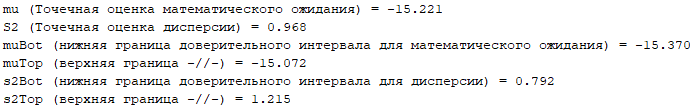
\includegraphics[scale=1]{inc/img/output.png}
\captionsetup{justification=centering}
	\caption{Поток вывода программы.}
	\label{img:output}	
\end{center}
\end{figure}

\item На координатной плоскости Oyn построить прямую $y=\hat \mu (\vec x_N)$, также графики функций $y=\hat \mu (\vec x_n), y= \underline \mu (\vec x_n), y =\overline \mu (\vec x_n)$ как функций объема n выборки, где n изменяется от 1 до N.

\begin{figure}[H]
\begin{center}
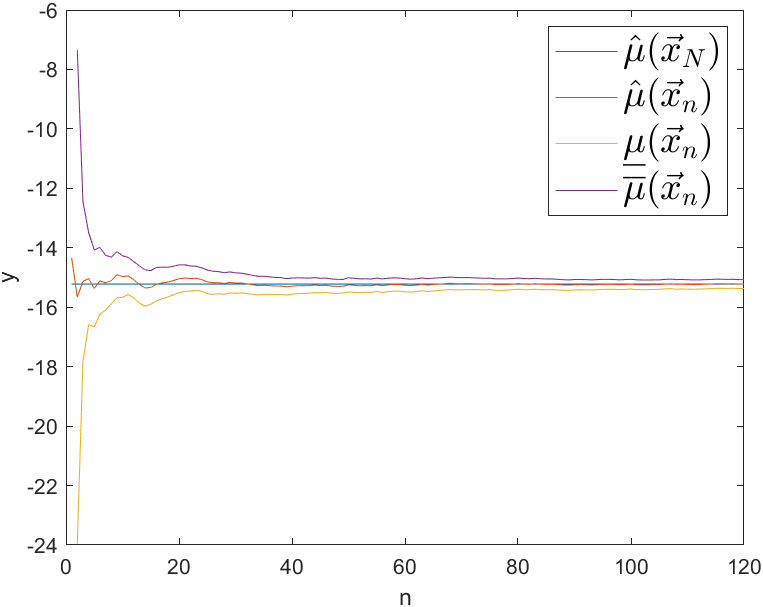
\includegraphics[scale=1]{inc/img/outputGraph.png}
\captionsetup{justification=centering}
	\caption{Прямая $y=\hat \mu (\vec x_N)$ и графики функций $y=\hat \mu (\vec x_n), y= \underline \mu (\vec x_n), y =\overline \mu (\vec x_n)$ как функций объема n выборки, где n изменяется от 1 до N.}
	\label{img:outputGraph}	
\end{center}
\end{figure}

\newpage

\item На координатной плоскости Ozn построить прямую $z=\hat S^2 (\vec x_N)$, также графики функций $z= S^2 (\vec x_n), z= \underline \sigma^2 (\vec x_n), z =\overline \sigma^2 (\vec x_n)$ как функций объема n выборки, где n изменяется от 1 до N.

\begin{figure}[H]
\begin{center}
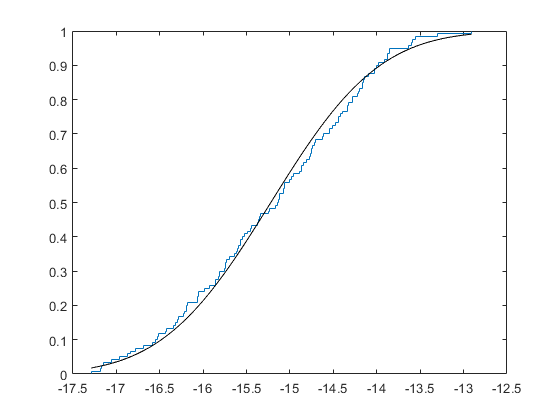
\includegraphics[scale=1]{inc/img/outputGraph2.png}
\captionsetup{justification=centering}
	\caption{Прямая $z=\hat S^2 (\vec x_N)$ и графики функций $z= S^2 (\vec x_n), z= \underline \sigma^2 (\vec x_n), z =\overline \sigma^2 (\vec x_n)$ как функций объема n выборки, где n изменяется от 1 до N.}
	\label{img:outputGraph2}	
\end{center}
\end{figure}

\begin{figure}[H]
\begin{center}
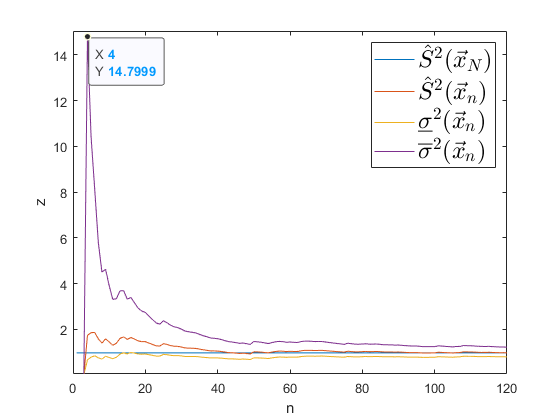
\includegraphics[scale=1]{inc/img/outputGraph3.png}
\captionsetup{justification=centering}
	\caption{Прямая $z=\hat S^2 (\vec x_N)$ и графики функций $z= S^2 (\vec x_n), z= \underline \sigma^2 (\vec x_n), z =\overline \sigma^2 (\vec x_n)$ как функций объема n выборки, где n изменяется от 1 до N.}
	\label{img:outputGraph3}	
\end{center}
\end{figure}

\begin{figure}[H]
\begin{center}
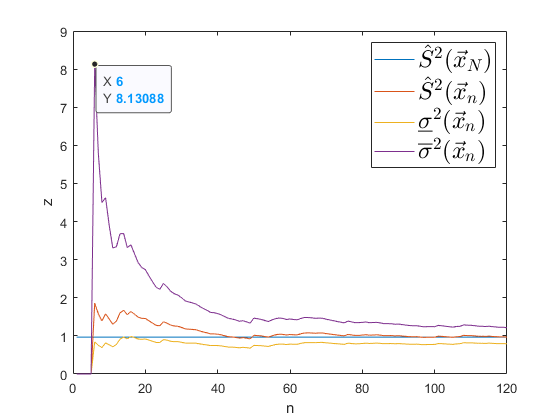
\includegraphics[scale=1]{inc/img/outputGraph4.png}
\captionsetup{justification=centering}
	\caption{Прямая $z=\hat S^2 (\vec x_N)$ и графики функций $z= S^2 (\vec x_n), z= \underline \sigma^2 (\vec x_n), z =\overline \sigma^2 (\vec x_n)$ как функций объема n выборки, где n изменяется от 1 до N.}
	\label{img:outputGraph4}	
\end{center}
\end{figure}

\end{enumerate}
\end{document}